\chapter{Conclusion}
\label{chapter:conclusion}
As a summary this dissertation, I focus on understanding the transport property of the heavy flavor in the strongly coupled quark-gluon plasma applying model-to-data comparison methodology, aiming for model improvements and uncertainty quantification.

A prerequisite for the study in an ``accurate'' modeling of the physical ingredients to be tested.
It is not so trivial to model the heavy quark transport that is coupled to an event-by-event fluctuating and evolving medium.
On the one hand, this is because the finite medium-induced radiation formation time at high energy is much greater than the mean-free-path in semi-classical transport equations, and can be comparable to the medium evolution time scales.
On the other hand, there are two compelling pictures regarding the heavy-quark-to-medium coupling: weakly coupled picture modeled by scatterings, and strongly coupled picture whose dynamics is often modeled by diffusion equations.
We developed a transport model for hard parton propagation in near equilibrium plasma. 
An improved treatment of LPM is implemented and it is shown to reduces to theoretical calculations in idealized infinite static medium limit, and captures qualitative features in a finite and evolving medium.
The model also treats the large and small momentum transfer processes with different strategies of few-body scattering and diffusion (plus diffusion-induced radiation) method, which grants flexible parametrization of diffusion-like deviations from leading order weakly coupled approach.

The transport in hot QGP stage fits into a more general ``transport'' picture including the initial production and high-virtuality evolution, hadronization near the transition temperature and decay and hadronic dynamics.
We identity a matching problem between the high-virtuality evolution and medium-induced evolution.
Currently, a unified formulation that smoothly connecting the virtuality shower and the in-medium shower is still missing, and we use a separation of phase-space to terminate vacuum showers at a scale ($Q^2$) where it is likely to receive similar amount of medium modifications to the transverse momentum ($\Delta k_\perp^2 \sim Q^2$).
The exact location of the separation scale is then treated as an uncertainty of the model.

Finally, we apply the Bayesian analysis to infer the model parameter distribution by comparing to heavy flavor measurements at both RHIC and the LHC.
The model parameters includes uncertainties such as in-medium coupling strength, energy loss starting time, match scale between vacuum and medium-induced shower, diffusion versus scattering model, as well as parametrized deviations from weakly coupled calculations.

\begin{figure}
\centering
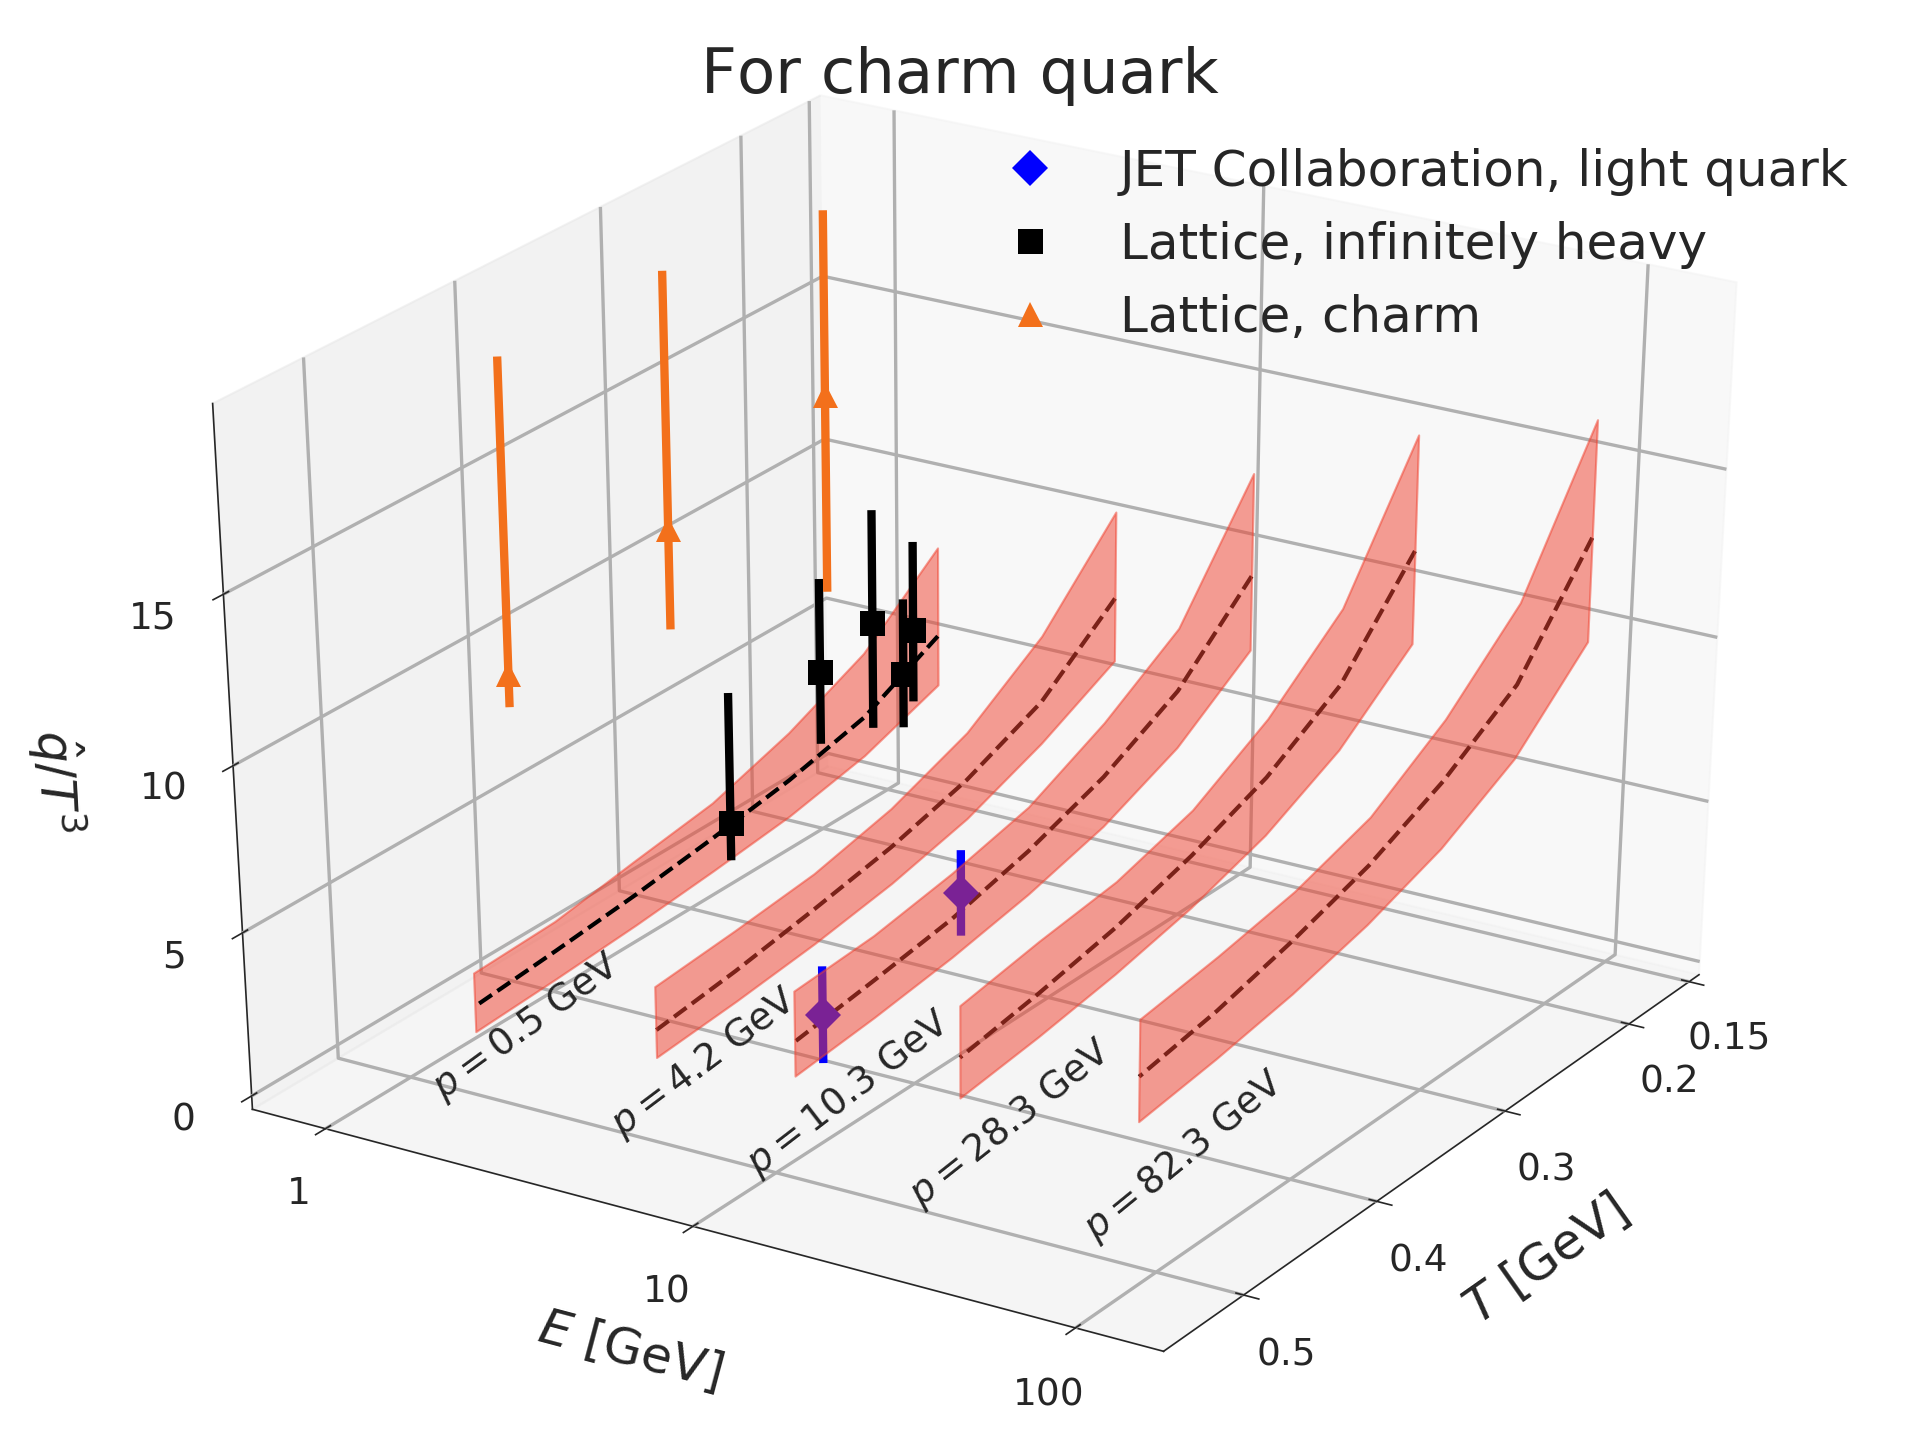
\includegraphics[width=.8\textwidth]{qhat_posterior_3D.png}
\caption{}
\label{fig:conlusion}
\end{figure}

We highlight the progress of this work in the conclusion figure \ref{fig:conlusion}.
It visualizes $90\%$ credible region of the energy and momentum dependence of the heavy quark momentum diffusion transport parameter $\hat{q}$ scaled by $T^3$.
We found $\hat{q}/T^3$ gradually increases with $\ln E$ and displays an enhancement near the critical temperature.
Studying heavy flavor helps to connect the knowledge of in-medium transport properties at very high momentum (light limit) and very low momentum (static sources limit).
At relatively high momentum $p\sim 10$ GeV, it is consistent to the light quark transport parameter extracted by the JET Collaboration (blue).
At low momentum $p\sim 0.5$ GeV, it is consistent with lattice calculations in the heavy quark limit (black).
Future study with improved flavor dependence may be needed to understand the impact of using the ``heavy' limit in dynamical model.
In the current present calibration, the effective in-medium strong coupling constant is about $0.3$, and only contribute a small fraction of the extracted $\hat{q}$ parameter.
The rest comes from the parametric contribution whose origin can be either perturbative or non-perturbative; either way, it suggests the necessity to model beyond leading order physics.

In conclusion, a transport modeling with perturbative based parton evolution with a parametric probe-medium interaction term is able to describe a wide range of open heavy flavor data to about 30\% level of accuracy.
The heavy quark transport properties as function of energy and temperature is consistent with early phenomenological studies and lattice calculation.
The present level model accuracy is still not enough to make the best use of future high-precision hard probe measurements in heavy-ion collisions []. 
We therefore summarize a few points of improvements in the end which may help to reduce or estimate the theoretical and modeling uncertainties.
\begin{itemize}
\item An interpolation formula between vacuum and medium-induced radiation. A calculation that connects virtuality evolution with in-medium time evolution will help to eliminated the matching scale uncertainty. Though for the present observable and $p_T$ range its effect is not strong, its treatment may impact more delicate jet observables.
\item Correlation among multiple emissions in the presence of medium. We have been neglecting the correlation among subsequent emissions in the ``modified transport model''. In the infinite medium limit, this is because the probability of overlapping emissions scales as $\tau_{1,f} R(\omega_2) \sim \tau_{1,f} \alpha_s/\tau_{2,f}$ which is suppressed by $\alpha_s$. But this higher order effect can be important since the phenomenological $\alpha_s$ is not small. There has been ongoing studies on this subject.
\item Off equilibrium correction to the linearized transport equation. One essential assumption in linearized transport model is that medium partons follow the local thermal distributions, even though the hydrodynamics is propagated with viscous corrections. In fact, the viscous correction and the momentum space anisotropy can be very large at early times of the hydrodynamic evolution. One need to understand how these off-equilibrium effects changes the interpretation of the transport parameter one extracted assuming full thermal equilibrium of partons.
\item Dynamical hadronization model and improved treatment of energy loss in the hadronic stage.
Our current hadronization model has the problem of pinching long distance physics into a sudden process. 
At low-$p_T$, the sudden recombination model breaks the detailed balance of the transport model and treating recombination model in a dynamical way would be more suitable.
At high-$p_T$, the problem is more severe, as the hadronization time scale is dilatation by the large boost. 
Moreover, the hadronic system near $T_c$ is still very dense, and it is inconsistent to apply the vacuum fragmentation function at the moment $T\sim T_c$.
One possible solution for those high-$p_T$ heavy quarks (the recombination process is negligible) is to continue their partonic transport into the hadronic phase, and finally apply the vacuum fragmentation function when the system is dilute enough.
Meanwhile, one can also study the energy loss in the dense hadronic system to extend the extracted transport parameter to the region below $T_c$.
\item A calibration with simultaneous tuning bulk and hard sector. The bulk medium calibration is performed by a separate analysis. With future high precision hard probe measurements, a simultaneous calibration of of both soft and hard sector would be interesting.
For example, we found that the number of binary collision as function of centrality is quite sensitive to the proton shape modeling in the Monte-Carlo Glauber model. The sensitivity of hard production to the number of binary collision may help the soft sector to improve the proton shape modeling. In turn, a better calibrated medium help to reduce the uncertainty in the hard parton energy loss.
\end{itemize}